\newpage
\hypertarget{subsec:fastGUI}{}
\subsection{FastCards in the GUI}
\genHeader

We hope you haven't forgotten about the GUI! Now that we have a new \texttt{card} type, let's quickly try editing our \texttt{box} instance so we can experiment
with them in our application.

\begin{itemize}
  
\item[$\blacktriangleright$] To review the details of creating instances, read Part II, Section 3 but for now, open \texttt{Box.xmi}, right-click on your
first partition, and create a new \texttt{FastCard} child element. Open the properties tab below, and edit the \texttt{back} and \texttt{face} values for
testing (Fig.~\ref{eclipse:fastCardProperties}). As you can see, it has all the same attributes as a standard \texttt{card}.

\vspace{0.5cm}

\begin{figure}[htbp]
\begin{center}
  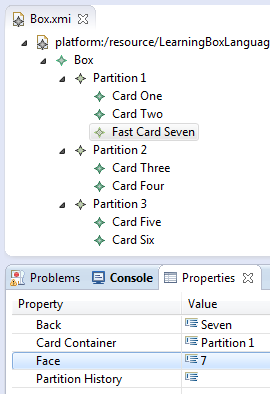
\includegraphics[width=0.4\textwidth]{eclipse_fastCardProperties}
  \caption{Creating and editing a new \texttt{FastCard} element}  
  \label{eclipse:fastCardProperties}
\end{center}
\end{figure}

\item[$\blacktriangleright$] Save your file, then open the GUI and try your extended \texttt{check} method. Experiment with making wrong and correct
guesses for both card types, paying attention their behaviour. If you've done everything right until this point, your newest \texttt{FastCard} should act
differently than its standard \texttt{card} counterparts.

\end{itemize}
